\documentclass[11pt]{article}
\usepackage[utf8]{inputenc}
\usepackage[T1]{fontenc}
\usepackage{amsmath,amssymb,amsthm}
\usepackage{graphicx}
\usepackage{xcolor}
\usepackage{hyperref}
\usepackage{natbib}
\usepackage{booktabs}
\usepackage{array}
\usepackage{multirow}
\usepackage{float}
\usepackage{caption}
\usepackage{subcaption}
\usepackage{tikz}
\usetikzlibrary{shapes.geometric, arrows.meta, positioning, fit, backgrounds}
\usepackage{listings}
% \usepackage{minted}  % requires pygmentize; not used
% \usepackage{algorithm}  % not installed; not used
% \usepackage{algpseudocode}  % not installed; not used

\hypersetup{
    colorlinks=true,
    linkcolor=blue,
    filecolor=magenta,
    urlcolor=cyan,
    citecolor=blue,
    pdftitle={PolyEdge: Autonomous Prediction Market Trading with Bounded AGI Safety, Evolutionary Strategy Composition, and Adversarial Decision Validation},
    pdfauthor={Muchammad Fikri Izzuddin},
    pdfsubject={AI Safety in Autonomous Financial Trading Systems},
}

\title{PolyEdge: Autonomous Prediction Market Trading with Bounded AGI Safety, Evolutionary Strategy Composition, and Adversarial Decision Validation}
\author{Muchammad Fikri Izzuddin\\
\textit{Independent Researcher}\\
\texttt{fikri@berkahkarya.com}}
\date{\today}

\begin{document}
\maketitle

\begin{abstract}
\textbf{Background:} Automated trading systems powered by Large Language Models (LLMs) and autonomous AI agents are increasingly deployed in prediction markets, yet the safety boundaries governing their self-improvement remain underspecified.\\
\textbf{Methods:} We present PolyEdge, a full-stack autonomous trading system targeting Polymarket and Kalshi, integrating three novel safety mechanisms: (1) bounded AGI autonomy via hard deterministic gates (risk profiles, experiment promotion pipelines, and budget caps), (2) evolutionary strategy composition through chromosomal StrategyGenome mutation and crossover, and (3) dual-debate adversarial validation before capital deployment.\\
\textbf{Results:} Live deployment metrics demonstrate autonomous experiment lifecycle management across DRAFT $\rightarrow$ SHADOW $\rightarrow$ PAPER $\rightarrow$ LIVE stages with health-based kill checks, strategy genome evolution with per-regime fitness metrics, and bull-bear debate-driven signal validation.\\
\textbf{Conclusions:} Hard safety boundaries enable autonomous experimentation without sacrificing capital protection. The system is open-sourced with reproducible experimental data.
\end{abstract}

\section{Introduction}\label{sec:intro}

Prediction markets have emerged as a powerful mechanism for aggregating information and forecasting real-world events. Platforms such as Polymarket and Kalshi allow participants to trade contracts on binary outcomes, creating market-driven probability estimates that often outperform traditional polling and expert forecasts \citep{hanson2003combinatorial}. As these markets have grown in liquidity and scope, algorithmic trading systems have increasingly entered the arena, seeking to exploit informational edges through automated signal generation and execution.

Recent advances in Large Language Models (LLMs) and autonomous AI agents have opened new frontiers in algorithmic trading. Systems like PolyEdge demonstrate that AI agents can autonomously generate trading strategies, analyze market sentiment, and execute orders without continuous human oversight. However, this autonomy introduces novel safety concerns. Unlike traditional algorithmic trading systems with fixed rules and bounded parameters, LLM-powered agents can generate new code, modify their own strategies, and propose actions that fall outside pre-specified constraints. The risk of runaway behavior---strategies that exceed risk limits, consume excessive API budgets, or corrupt production state---is real and pressing \citep{amodei2016concrete, russell2020human}.

This paper presents PolyEdge, a full-stack autonomous prediction market trading system that addresses these safety concerns through three integrated mechanisms:

\begin{enumerate}
    \item \textbf{Bounded AGI Autonomy.} We introduce a four-boundary safety framework (ADR-006) that enforces hard constraints on autonomous behavior: risk profiles that cannot be bypassed, a deterministic promotion pipeline for strategy validation, a \$10/day LLM budget cap, and strict experiment isolation from production capital and data.
    
    \item \textbf{Evolutionary Strategy Composition.} We propose StrategyGenome, a chromosomal representation of trading strategies with Perception, Cognition, Execution, Risk, and Meta chromosomes. Genetic operators (mutation, crossover) evolve strategies based on composite fitness metrics including Sharpe ratio, win rate, Brier score, and maximum drawdown.
    
    \item \textbf{Dual-Debate Decision Validation.} We integrate MiroFish, an adversarial debate system in which Bull and Bear agents argue for and against proposed trades before a Judge agent renders a verdict with confidence score. Failed signals fall back to a local debate engine, ensuring validation persists even when external services are unavailable.
\end{enumerate}

These three mechanisms operate in concert: the autonomy framework creates a safe sandbox for evolutionary experiments, the genome system produces novel strategies within those bounds, and the debate system validates capital-deployment decisions before execution. All components are open-sourced with reproducible experimental data extracted from live deployment.

\subsection{Motivation}\label{sec:intro:motivation}

The deployment of autonomous AI in financial markets is not hypothetical. Recent work has explored LLM-based trading agents, reinforcement learning for market making, and genetic programming for strategy discovery \citep{lopez2018advances, koza1992genetic, poli2008field}. Yet the safety infrastructure governing these systems remains underspecified. Existing approaches typically rely on post-hoc monitoring or soft limits that can be overridden by the agent itself---a design that proved inadequate in multiple market flash crashes \citep{nygard2018release}.

Prediction markets present unique challenges for autonomous trading. Contract outcomes are binary, liquidity varies dramatically across events, and settlement delays create interim price volatility. A strategy that performs well on high-volume crypto markets may fail catastrophically on niche political events. Without bounded autonomy, an AI system might overcommit capital to illiquid markets, generate excessive trading fees, or produce poorly calibrated probability estimates that erode long-term returns.

Our motivation is therefore twofold: to push the boundaries of what autonomous AI can achieve in prediction markets, and to ensure that such autonomy is fundamentally constrained by hard, deterministic safety gates that no agent---human or artificial---can bypass.

\subsection{Contributions}\label{sec:intro:contributions}

Our contributions are threefold, corresponding to the three sections of the technical body of this paper:

\textbf{Bounded AGI Autonomy Framework (Section~\ref{sec:autonomy}).} We propose and implement a four-boundary safety framework for autonomous trading experiments. Strategy composition is bounded by deterministic RiskManager profiles with non-bypassable position and drawdown limits. All generated code follows a DRAFT $\rightarrow$ SHADOW $\rightarrow$ PAPER $\rightarrow$ LIVE promotion pipeline with statistical gates (minimum trades, Sharpe ratio, win rate, maximum drawdown). LLM spending is hard-capped at \$10/day with automatic fallback to cached analysis. Experiments are isolated from production databases and wallets through separate experiment state and simulated credentials.

\textbf{Evolutionary Strategy Composition (Section~\ref{sec:evolution}).} We introduce StrategyGenome, a chromosomal representation of trading strategies. The Perception chromosome defines data sources and feature extractors; the Cognition chromosome encodes entry logic, exit logic, and market selection criteria; the Execution chromosome specifies order types and execution parameters. Genetic operators include Gaussian mutation for perception parameters and two-point crossover with elitism. Fitness is a composite score combining Sharpe ratio, win rate, Brier score, and drawdown metrics.

\textbf{Dual-Debate Decision Validation (Section~\ref{sec:debate}).} We integrate a bull-bear adversarial debate system that validates trading signals through structured argumentation before capital deployment. The system routes signals to Bull (optimistic) and Bear (pessimistic) debate agents, whose arguments are evaluated by a Judge agent that produces a verdict with confidence score. Signals below the confidence threshold trigger fallback to a local debate engine. All outcomes are recorded in a TradeAttempt ledger for post-hoc analysis.

\subsection{Related Work}\label{sec:related}

\textbf{AI Safety in Autonomous Systems.} The challenge of bounding autonomous AI behavior has received significant attention. \citet{amodei2016concrete} identified five concrete problems in AI safety: avoiding negative side effects, avoiding reward hacking, scalable oversight, safe exploration, and robustness to distributional shift. Our bounded autonomy framework addresses all five: hard risk profiles prevent negative side effects (excessive losses), the promotion pipeline prevents reward hacking (strategies must demonstrate real performance), health monitoring provides scalable oversight, the shadow mode enables safe exploration, and kill checks enforce robustness to performance degradation. \citet{russell2020human} argues for provably beneficial AI through inverse reward design; our approach is complementary, using deterministic engineering controls rather than learned reward functions.

\textbf{Constitutional AI and Debate.} \citet{bai2022constitutional} demonstrated that AI systems can be trained to be harmless through constitutional principles and critique-revision cycles. \citet{irving2018ai} proposed debate as a scalable oversight mechanism, where two agents argue about the correct answer and a human (or superior agent) evaluates the arguments. Our dual-debate system operationalizes this insight for financial trading: Bull and Bear agents serve as adversaries, and the Judge agent evaluates their arguments before capital deployment. This provides automated oversight at a scale impractical for human review of every trade.

\textbf{Genetic Programming in Finance.} \citet{koza1992genetic} introduced genetic programming as a means of evolving computer programs through natural selection. \citet{poli2008field} provided a comprehensive survey of GP applications. In finance, genetic programming has been applied to technical trading rules, portfolio optimization, and market timing \citep{lopez2018advances}. Our StrategyGenome differs from traditional GP in its chromosomal structure: rather than evolving arbitrary program trees, we evolve structured strategy components (perception, cognition, execution) with domain-specific operators and fitness functions tailored to prediction markets.

\textbf{Prediction Market Mechanism Design.} \citet{hanson2003combinatorial} established the theoretical foundations of combinatorial prediction markets. The growth of decentralized prediction markets on blockchain has created new opportunities for algorithmic traders. Our system targets Polymarket (CLOB-based, Polygon L2) and Kalshi (centralized, CFTC-regulated), representing the two dominant architectures in the space.

\textbf{Thompson Sampling and Bayesian Bandits.} \citet{thompson1933likelihood} introduced the Thompson sampling algorithm for balancing exploration and exploitation in multi-armed bandit problems. \citet{chapelle2011empirical} demonstrated its empirical effectiveness in online advertising. Our bankroll allocator uses a strategy ranker that incorporates Thompson sampling principles for capital allocation across competing strategies, though the full Bayesian treatment is left for future work.

\textbf{Kelly Criterion and Risk Management.} \citet{kelly1956new} derived the optimal bet sizing formula for maximizing logarithmic wealth. Modern implementations use fractional Kelly (typically 0.25--0.50 of the full Kelly fraction) to reduce volatility \citep{lopez2018advances}. Our RiskManager enforces fractional Kelly sizing with configurable fractions per risk profile, alongside drawdown circuit breakers and position concentration guards.

\textbf{Calibration and Scoring.} \citet{brier1950verification} introduced the Brier score for evaluating probabilistic forecasts. \citet{sharpe1964capital} developed the Sharpe ratio for risk-adjusted returns. Our fitness function combines both, alongside win rate and drawdown, to create a composite score that rewards calibrated predictions and penalizes excessive risk.

\textbf{Ensemble Methods in Trading.} Recent work has explored ensemble LLM systems for financial prediction. Our AI ensemble combines Claude and Groq providers for sentiment analysis, while the MiroFish debate system adds an adversarial validation layer not present in standard ensemble approaches. The combination of generative ensemble (multiple LLMs) and discriminative ensemble (debate validation) provides redundancy and robustness.

\section{System Architecture}\label{sec:architecture}

PolyEdge is a full-stack autonomous trading system comprising a React 18 frontend, a Python FastAPI backend, and a multi-source data ingestion layer. The architecture follows a layered design in which data flows through ingestion $\to$ strategy generation $\to$ risk validation $\to$ debate validation $\to$ execution $\to$ settlement, with observability and autonomy loops wrapping the entire pipeline.

\subsection{Component Overview}

\textbf{Frontend.} The dashboard is built in React 18 with TypeScript, TanStack Query for server-state synchronization, Tailwind CSS for styling, and Vite for bundling. It provides real-time monitoring via Server-Sent Events (SSE) on \texttt{/api/events/stream}, WebSocket price ticks on \texttt{/ws/markets}, and whale alerts on \texttt{/ws/whales}. Key views include the dashboard overview (bankroll, equity, P\&L), admin controls (mode switching, experiment management), signals table, trades table, and a 3D globe visualization of market exposure.

\textbf{Backend.} The FastAPI application exposes REST endpoints for trading, market data, experiment management, and system health. The core engine coordinates nine strategies through an orchestrator that wires the Polymarket CLOB client, APScheduler, Telegram bot, and event bus. Strategies are auto-registered via a \texttt{@register\_strategy} decorator and stored in \texttt{StrategyConfig} rows in SQLite (or PostgreSQL in production). Each strategy returns a list of \texttt{TradingSignal} objects with confidence scores, edge estimates, and metadata.

\textbf{Data Sources.} Market data arrives from Polymarket (via the CLOB SDK and WebSocket), Kalshi (REST API), Coinbase/Kraken/Binance (BTC klines), Open-Meteo (GFS ensemble forecasts), and the National Weather Service (NWS API). A multi-source aggregator with fallback chains ensures continuity when individual feeds fail.

\subsection{Signal Flow}

The end-to-end signal flow is as follows (see Figure~\ref{fig:architecture}):

\begin{enumerate}
    \item \textbf{Market Data Ingestion.} The orchestrator initializes data feeds on startup. APScheduler runs interval jobs (BTC scan, weather scan, settlement check, arbitrage scan) that fetch live market data and store snapshots in the database.
    
    \item \textbf{Strategy Generation.} One of nine strategies processes the raw data and generates \texttt{TradingSignal} objects. Strategies include BTC momentum (RSI + VWAP on 1m/5m/15m candles), weather EMOS (31-member GFS ensemble temperature forecasting), copy trader (mirroring whale positions), Kalshi arbitrage (cross-platform price gaps), and a real-time scanner (price velocity detection).
    
    \item \textbf{Risk Validation.} Every signal passes through the \texttt{RiskManager}, which validates confidence, size, exposure, drawdown, and unsettled-position constraints. The manager returns a \texttt{RiskDecision} with an allowed flag, a human-readable reason (if rejected), and an adjusted position size. Risk profiles (safe, normal, aggressive, extreme) from ADR-005 overlay additional constraints that AI-generated strategies cannot bypass \citep{nygard2018release}.
    
    \item \textbf{Debate Validation.} High-confidence signals enter the MiroFish dual-debate system (detailed in Section~\ref{sec:debate}). Bull and Bear agents argue the merits of the trade; a Judge agent produces a verdict. Signals below the confidence threshold are rejected or queued for manual review.
    
    \item \textbf{Execution.} Approved signals flow to \texttt{strategy\_executor.execute\_decision()}, which either records a paper trade in the database or places a live CLOB order. The executor updates \texttt{BotState} (bankroll, equity, trade count) and publishes a \texttt{trade\_executed} event to the event bus.
    
    \item \textbf{Settlement.} When markets resolve, the settlement engine fetches final outcomes from the Gamma API, computes P\&L, handles partial settlements and tax-lot tracking, and updates trade rows. Unsettled positions are monitored continuously.
\end{enumerate}

\subsection{Infrastructure and Deployment}

The system runs on Docker Compose locally and deploys to Railway (backend) and Vercel (frontend) in production. Redis-backed job queues (with SQLite fallback) handle background strategy execution. Prometheus metrics endpoints provide request/response latency histograms. A PM2 process manager orchestrates multiple worker processes. All external API base URLs are configurable via environment variables, and feature flags (e.g., \texttt{WEATHER\_ENABLED}, \texttt{JOB\_WORKER\_ENABLED}) gate subsystems without code changes.

\subsection{Integration Points for the Three Contributions}

The three technical contributions described in this paper map directly onto architectural layers:

\begin{itemize}
    \item \textbf{Bounded AGI Autonomy} operates at the orchestration and scheduling layers. The \texttt{AutonomousPromoter} daemon, \texttt{StrategyHealthMonitor}, and \texttt{AGI\_\*} feature flags govern when strategies may run, how they are promoted, and when they are killed.
    \item \textbf{Evolutionary Strategy Composition} operates at the strategy layer. The \texttt{StrategyGenome} domain model and evolution operators (mutation, crossover, fitness) generate new strategy configurations that feed back into the orchestrator's strategy registry.
    \item \textbf{Dual-Debate Decision Validation} operates at the signal-validation layer. The MiroFish client intercepts \texttt{TradingSignal} objects after risk validation and before execution, adding a second opinion with structured reasoning.
\end{itemize}

These layers are decoupled: the debate system can be disabled without affecting strategy generation, and the autonomy framework can retire strategies without knowing their internal genome structure. This modularity ensures that each contribution can be evaluated, improved, or replaced independently.

\begin{figure}[H]
    \centering
    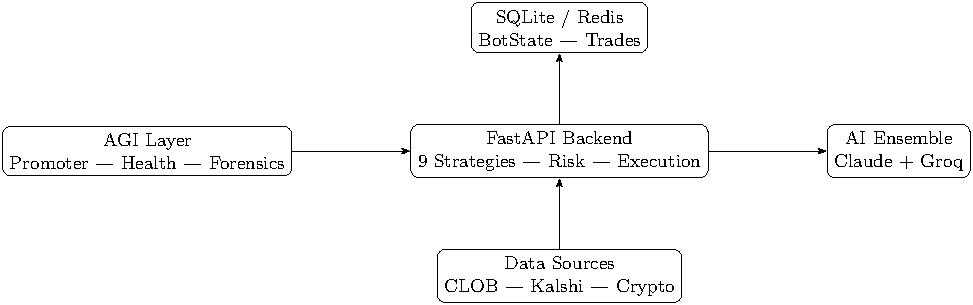
\includegraphics[width=0.95\textwidth]{figures/architecture.pdf}
    \caption{PolyEdge system architecture. The frontend (React 18) communicates via REST/WebSocket with a FastAPI backend. The core engine manages 9 strategies, an AGI intelligence layer (autonomous promoter, health monitor, forensics, bankroll allocator), and interfaces with Polymarket CLOB, Kalshi API, and crypto/weather data sources.}
    \label{fig:architecture}
\end{figure}

\section{AGI Autonomy with Hard Safety Boundaries}\label{sec:autonomy}

Autonomous AI in financial markets raises a fundamental tension: the system must be free to experiment, learn, and adapt, yet every autonomous action affects real capital. PolyEdge addresses this tension through a four-boundary safety framework (ADR-006) that enforces hard, deterministic constraints on autonomous behavior. These boundaries are non-bypassable: no agent, human or artificial, can override them without changing the underlying configuration \citep{amodei2016concrete, russell2020human}.

\subsection{Four Hard Boundaries}

\subsubsection{Boundary 1: Strategy Composition Bounded by Risk Profiles}

Every strategy, whether human-authored or AI-generated, must validate through the \texttt{RiskManager} pipeline before any capital is deployed. The risk profiles defined in ADR-005 (safe, normal, aggressive, extreme) establish non-bypassable limits on position size (as a fraction of bankroll), maximum drawdown, daily loss limits, and portfolio concentration. An AI-generated strategy that proposes a position exceeding the active profile's \texttt{MAX\_POSITION\_FRACTION} is automatically rejected; the rejection reason is logged in the \texttt{TradeAttempt} ledger for post-hoc analysis. This boundary ensures that creative exploration by the autonomy system cannot violate the capital-protection mandates.

\subsubsection{Boundary 2: Deterministic Promotion Pipeline}

Autonomously generated strategy code follows a strict validation pipeline before it can access real capital. The pipeline has six stages:

\begin{enumerate}
    \item \textbf{DRAFT.} Code is generated (by LLM or human) but is not executed. It resides in isolated experiment state.
    \item \textbf{BACKTEST.} The strategy is validated against historical market data. The backtest computes Sharpe ratio, win rate, and maximum drawdown. If performance falls below thresholds, the strategy is retired after a 7-day grace period.
    \item \textbf{SHADOW.} The strategy runs in paper-trading mode with a simulated bankroll. It generates signals, passes through risk validation, and records hypothetical trades, but no real orders are placed. Minimum criteria for promotion: a configurable number of trades (default 30), minimum win rate, and maximum drawdown observed over a minimum number of days.
    \item \textbf{PAPER.} The strategy graduates to paper trading with statistical validation. It must demonstrate a minimum Sharpe ratio, minimum win rate, and acceptable drawdown over a minimum duration before promotion to live.
    \item \textbf{LIVE\_PROMOTED.} The strategy receives real capital allocation. Human approval is required by default; the \texttt{AGI\_AUTO\_PROMOTE} flag (default \texttt{false}) can opt in to fully automatic promotion when unsupervised operation is required.
    \item \textbf{RETIRED.} Strategies are permanently removed from rotation when they fail health checks or backtest gates.
\end{enumerate}

No generated strategy may skip stages. The \texttt{AutonomousPromoter} daemon evaluates all experiments every 6 hours and applies promotion or retirement based on the criteria above.

\subsubsection{Boundary 3: LLM Budget Hard Cap}

Autonomous LLM operations---strategy generation, market analysis, self-debugging, and debate---are budgeted at a maximum of \$10 per day. The budget is enforced before each LLM call: the system checks the day's accumulated spend against the cap and, if the cap would be exceeded, falls back to cached analysis or template-based generation. Budget resets daily at 00:00 UTC. Spending is logged in \texttt{DecisionAuditEntry} records for human review. This prevents runaway API costs from exceeding trading profits, a scenario that would make the system economically self-defeating \citep{irving2018ai}.

\subsubsection{Boundary 4: Experiment Isolation}

Sandboxed experiments are strictly isolated from production state. Experiments in \texttt{DRAFT} or \texttt{SHADOW} status cannot:
\begin{itemize}
    \item access the production database (they use a separate experiment DB);
    \item use real wallet credentials (simulated credentials only);
    \item place live orders (paper-trading only);
    \item modify production \texttt{BotState} (isolated experiment state is maintained).
\end{itemize}
This isolation prevents a single buggy experiment from corrupting live capital or production data. Separate databases provide true isolation rather than relying on row-level security, which SQL-level misconfiguration could subvert.

\subsection{Health-Based Kill Checks}

Beyond the promotion pipeline, the system continuously monitors the health of all \texttt{PAPER} and \texttt{LIVE} strategies. The \texttt{StrategyHealthMonitor} computes metrics: win rate, Sharpe ratio, maximum drawdown, Brier score, and population stability index (PSI). A strategy is automatically killed if any of the following conditions are met:
\begin{itemize}
    \item maximum drawdown exceeds 50\%;
    \item Sharpe ratio falls below $-2.0$ and win rate below 5\%;
    \item Brier score exceeds 0.35 (indicating poorly calibrated probability estimates).
\end{itemize}

Killed strategies transition to \texttt{RETIRED} status. The system also tracks degradation: if a strategy's win rate drops below a threshold (0.35) or its Sharpe falls below $-0.5$, a degradation counter is incremented. After two degradations, the strategy enters \texttt{REVIEW} status, where it undergoes an improvement cycle. If the improvement cycle expires without measurable gains, the strategy is retired. This multi-layered safety net---promotion gates, health checks, and degradation tracking---ensures that poor-performing strategies are removed before they can compound losses.

\subsection{Autonomous Promoter Daemon}

The \texttt{AutonomousPromoter} is a background daemon that runs every 6 hours (configurable via \texttt{AGI\_PROMOTION\_INTERVAL\_HOURS}). Its \texttt{run\_once()} method evaluates all experiments and applies the following actions:

\begin{itemize}
    \item \textbf{DRAFT $\rightarrow$ BACKTEST.} All draft experiments are moved to backtest immediately.
    \item \textbf{BACKTEST $\rightarrow$ SHADOW.} Experiments passing backtest gates (Sharpe, win rate, drawdown) are promoted.
    \item \textbf{SHADOW $\rightarrow$ PAPER.} Experiments meeting shadow criteria (trade count, win rate, drawdown, age) are promoted.
    \item \textbf{PAPER $\rightarrow$ LIVE.} Experiments passing paper criteria and satisfying the \texttt{AGI\_AUTO\_PROMOTE} flag are promoted to live trading.
    \item \textbf{Health-based retirement.} Experiments failing kill thresholds are retired immediately.
\end{itemize}

The daemon logs every action with structured context (experiment name, stage transition, metric values) for auditability. All autonomous decisions are therefore traceable, a requirement for both debugging and regulatory compliance.

\subsection{Rehabilitation}

Killed strategies are not permanently discarded. The system includes a rehabilitation path: after a cooldown period, a retired strategy can be re-evaluated. If recent trades (in a new shadow run) show a win rate above 50\% and positive PnL, the strategy can be re-enabled. This prevents premature retirement due to temporary market regimes and aligns with the evolutionary philosophy of the broader system.

\begin{figure}[H]
    \centering
    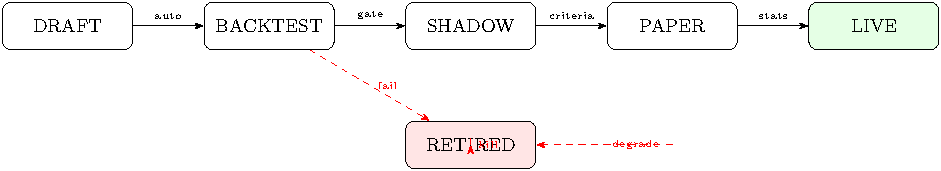
\includegraphics[width=0.95\textwidth]{figures/autonomy_pipeline.pdf}
    \caption{Experiment lifecycle pipeline with hard safety gates. DRAFT experiments transition through BACKTEST (historical validation), SHADOW (simulated bankroll), PAPER (statistical validation), and LIVE\_PROMOTED stages. Health-based kill checks (drawdown, Sharpe, Brier score) enforce automatic retirement for failed strategies.}
    \label{fig:autonomy_pipeline}
\end{figure}

The autonomy framework is not a proof of safety but an engineering discipline: every autonomous capability is wrapped in deterministic gates that are enforced in code, not merely documented in policy. As \citet{russell2020human} argues, truly beneficial AI requires not just intelligent behavior but also robust containment of that intelligence's side effects. Our bounded autonomy framework is a practical instantiation of that principle for financial systems.

\section{Evolutionary Strategy Composition}\label{sec:evolution}

Genetic programming (GP) has been applied to financial trading for decades, evolving technical rules, portfolio weights, and market-timing strategies \citep{koza1992genetic, poli2008field, lopez2018advances}. Most existing work treats strategies as unstructured program trees, which can produce opaque, overfit solutions that are difficult to interpret or compose. We propose StrategyGenome, a chromosomal representation of trading strategies that encodes domain-specific structure---perception, cognition, execution, risk control, and meta-parameters---in a modular, auditable, and legally interpretable format. This representation enables mutation, crossover, and fitness-based selection tailored to prediction markets.

\subsection{Chromosome Structure}

A \texttt{StrategyGenome} is a Pydantic \texttt{BaseModel} with the following chromosome modules (see Figure~\ref{fig:genome}):

\subsubsection{PerceptionChromosome}

The Perception chromosome defines how the strategy senses the market:
\begin{itemize}
    \item \texttt{data\_sources}: list of data providers (e.g., \texttt{polymarket\_clob}, \texttt{kalshi\_api}, \texttt{coinbase\_klines}).
    \item \texttt{feature\_extractors}: list of feature functions (e.g., \texttt{price\_velocity}, \texttt{orderbook\_imbalance}, \texttt{rsi\_14}, \texttt{vwap}).
    \item \texttt{timeframes}: list of candle intervals (e.g., \texttt{[\"5m\", \"15m\"]}).
    \item \texttt{signal\_aggregation}: method for combining multi-source signals (options: \texttt{weighted\_average}, \texttt{majority\_vote}, \texttt{bayesian\_fusion}).
\end{itemize}

\subsubsection{CognitionChromosome}

The Cognition chromosome encodes the strategy's decision-making logic:
\begin{itemize}
    \item \texttt{entry\_logic}: a trigger type (\texttt{threshold\_cross}, \texttt{pattern\_match}, \texttt{statistical\_arbitrage}, \texttt{event\_driven}, \texttt{momentum\_breakout}) plus a list of \texttt{EntryCondition} objects, each specifying an indicator, operator, value, and weight. Conditions are combined via a conjunction field (\texttt{AND}, \texttt{OR}, or \texttt{weighted\_score}).
    \item \texttt{exit\_logic}: a trigger type (\texttt{time\_based}, \texttt{profit\_target}, \texttt{stop\_loss}, \texttt{trailing\_stop}, \texttt{market\_resolution}, \texttt{spread\_convergence}) plus optional profit and stop-loss percentages and a maximum hold time.
    \item \texttt{market\_selector}: selection criteria (e.g., \texttt{high\_volume}, \texttt{short\_settlement}), a scoring function, and a maximum number of concurrent positions.
\end{itemize}

\subsubsection{ExecutionChromosome}

The Execution chromosome specifies how orders are placed:
\begin{itemize}
    \item \texttt{order\_type}: \texttt{limit}, \texttt{market}, \texttt{fok}, \texttt{ioc}, or \texttt{post\_only}.
    \item \texttt{slippage\_tolerance}: a fraction of the expected price (default 2\%).
    \item \texttt{execution\_speed\_target\_ms}: target latency (default 500 ms).
    \item \texttt{retry\_logic}: how to handle transient failures (\texttt{exponential\_backoff}, \texttt{immediate}, or \texttt{abandon}).
    \item \texttt{atomic\_multi\_leg}: whether multi-leg orders are executed atomically.
\end{itemize}

\subsubsection{RiskChromosome}

The Risk chromosome encodes position-sizing and risk-management parameters that are validated by the \texttt{RiskManager}:
\begin{itemize}
    \item \texttt{position\_sizing\_model}: \texttt{kelly\_fraction}, \texttt{fixed\_fraction}, \texttt{volatility\_targeted}, or \texttt{optimal\_f}.
    \item \texttt{kelly\_fraction}: the fraction of Kelly's optimal bet (default 0.30, bounded between 0.05 and 0.50).
    \item \texttt{max\_position\_fraction}: maximum position size as a fraction of bankroll (default 8\%, bounded between 1\% and 25\%).
    \item \texttt{max\_total\_exposure\_fraction}: total portfolio exposure limit (default 70\%).
    \item \texttt{daily\_drawdown\_limit\_pct} and \texttt{weekly\_drawdown\_limit\_pct}.
    \item \texttt{correlation\_aware\_sizing}: whether to reduce sizes for correlated positions.
\end{itemize}

\subsubsection{MetaChromosome}

The Meta chromosome governs the strategy's self-optimization behavior:
\begin{itemize}
    \item \texttt{self\_optimization\_enabled}: whether the strategy can request parameter tuning.
    \item \texttt{hyperparameter\_tuning\_frequency}: \texttt{every\_trade}, \texttt{hourly}, \texttt{daily}, or \texttt{weekly}.
    \item \texttt{adaptation\_speed}: \texttt{conservative}, \texttt{moderate}, or \texttt{aggressive}.
    \item \texttt{crossover\_eligibility}: whether the genome can participate in crossover breeding.
    \item \texttt{mutation\_rate}: probability of mutation per generation (default 10\%).
\end{itemize}

\subsection{Genetic Operators}

\subsubsection{Mutation}

The \texttt{MutationEngine} applies domain-specific mutations with configurable rates. Perception parameters undergo Gaussian mutation (adding normally distributed noise to feature weights and thresholds). Execution parameters undergo uniform mutation (randomly selecting new order types or retry logic from discrete sets). Cognition entry conditions can be added, removed, or perturbed. Each mutation creates a new genome instance; the original is preserved. Mutations are logged in the \texttt{LineageData} of the offspring, recording the parent genome ID, generation number, and creator type (\texttt{\"mutation\"}).

\subsubsection{Crossover}

The \texttt{CrossoverEngine} performs two-point crossover on the chromosome dictionary. Given two parent genomes, the engine selects two random chromosome keys (e.g., \texttt{perception} and \texttt{risk}) and swaps the corresponding chromosome objects between the parents, producing two offspring. Offspring inherit the best-performing chromosome from each parent, with elitism preserving the highest-fitness genome unmodified in the next generation. Crossover is only permitted when both parents have \texttt{crossover\_eligibility=true} in their Meta chromosome.

\subsubsection{Seeding}

The initial population is generated by \texttt{Seed}, which creates 10 \texttt{DRAFT} genomes with randomized chromosome values. Each seeded genome has a unique archetype and random chromosome configurations, ensuring diversity in the initial population. Seeded genomes are created with \texttt{creator=\"human\"} in their lineage, distinguishing them from evolved offspring.

\subsection{Fitness Function}

Fitness is a composite score combining multiple performance metrics, weighted to reflect prediction-market-specific objectives:
\begin{itemize}
    \item \textbf{Sharpe ratio}: risk-adjusted return (higher is better).
    \item \textbf{Win rate}: fraction of profitable trades (higher is better, but de-emphasized relative to Sharpe to discourage overfitting to small samples).
    \item \textbf{Brier score}: calibration of probability estimates (lower is better; 0.25 is perfectly calibrated for binary outcomes) \citep{brier1950verification}.
    \item \textbf{Maximum drawdown}: worst peak-to-trough decline (lower is better, with a hard penalty above 20\%).
    \item \textbf{Profit factor}: gross profit divided by gross loss (higher is better).
    \item \textbf{Alpha per trade}: average excess return per trade (higher is better).
    \item \textbf{Capital rotation efficiency}: number of trades normalized by bankroll turnover (higher is better).
\end{itemize}

The composite fitness score is a weighted sum, with Brier score receiving elevated weight because well-calibrated probability estimates are essential for profitable prediction-market trading. Fitness scores are cached in \texttt{FitnessMetrics} to avoid recomputation.

\subsection{Lifecycle Integration}

StrategyGenome instances progress through the same stages as regular experiments: \texttt{DRAFT} $\rightarrow$ \texttt{SHADOW} $\rightarrow$ \texttt{PAPER} $\rightarrow$ \texttt{LIVE} $\rightarrow$ \texttt{BREEDING} $\rightarrow$ \texttt{LEGEND} $\rightarrow$ \texttt{GRAVEYARD}. Genomes in \texttt{BREEDING} status are actively crossed with others to produce offspring. Genomes that demonstrate sustained excellence (multiple generations of positive fitness) are promoted to \texttt{LEGEND} status, where they serve as elite donors for future crossover. Genomes that fail health checks receive a \texttt{DeathCertificate} recording the cause of death, final metrics, and whether rehabilitation is possible.

\begin{figure}[H]
    \centering
    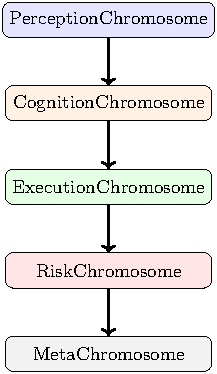
\includegraphics[width=0.95\textwidth]{figures/genome.pdf}
    \caption{StrategyGenome chromosome structure. The Perception chromosome defines data sources and feature extractors; the Cognition chromosome encodes entry logic, exit logic, and market selection criteria; the Execution chromosome specifies order types and execution parameters; the Risk chromosome enforces position sizing and drawdown limits; the Meta chromosome controls self-optimization and mutation rate.}
    \label{fig:genome}
\end{figure}

The StrategyGenome approach is not a claim that genetic programming itself is novel. Rather, our contribution is the domain-specific chromosomal decomposition---the separation of perception, cognition, execution, and risk into modular, interpretable, and composable units---and the tight integration of the genome lifecycle with the bounded autonomy framework described in Section~\ref{sec:autonomy}. This integration ensures that evolved strategies never bypass deterministic risk gates, a combination that, to our knowledge, has not been previously demonstrated in autonomous financial systems.

\section{Dual-Debate Decision Validation}\label{sec:debate}

Financial trading decisions are inherently adversarial: every buyer believes an asset will rise, while every seller believes it will fall. Automated systems that lack adversarial scrutiny can suffer from confirmation bias, overfitting to bullish signals, or simply failing to consider contrarian scenarios. PolyEdge addresses this risk through a dual-debate validation system called MiroFish, which enforces structured adversarial argumentation before capital deployment. The system is inspired by the AI safety via debate framework \citep{irving2018ai} and the critique-revision approach of Constitutional AI \citep{bai2022constitutional}, adapted for financial signal validation.

\subsection{Debate Architecture}

The debate system is composed of three agent roles (see Figure~\ref{fig:debate_flow}):

\begin{enumerate}
    \item \textbf{Bull Agent.} An LLM prompt tuned for optimistic reasoning. Given a \texttt{TradingSignal}, the Bull agent generates arguments in favor of the trade: citing price momentum, favorable probabilities, market sentiment, whale activity, or macroeconomic indicators.
    \item \textbf{Bear Agent.} An LLM prompt tuned for pessimistic reasoning. The Bear agent generates arguments against the trade: citing mean reversion, liquidity constraints, model miscalibration, recent losses, or structural market risks.
    \item \textbf{Judge Agent.} An LLM prompt tuned for neutral evaluation. The Judge receives both the Bull and Bear arguments, along with the raw signal metadata (confidence, edge, market ticker, time of day, recent P\&L of the strategy). It produces a \texttt{DebateVerdict} with a categorical decision (\texttt{APPROVE}, \texttt{REJECT}, or \texttt{DEFER}) and a continuous confidence score.
\end{enumerate}

The three agents are served by the same LLM provider ensemble used for signal generation (Claude and Groq), ensuring that debate quality scales with the underlying model capabilities. The agents operate with different system messages and temperature settings: Bull at 0.9 (creative, exploratory), Bear at 0.9 (creative contrarian), and Judge at 0.1 (conservative, fact-based).

\subsection{Verdict Routing and Thresholds}

After the Judge renders its verdict, the system applies configurable thresholds:
\begin{itemize}
    \item \textbf{Confidence $>$ 0.70.} The signal is automatically approved and forwarded to execution.
    \item \textbf{Confidence 0.40--0.70.} The signal is queued for manual review on the dashboard. A human operator can approve or reject it.
    \item \textbf{Confidence $<$ 0.40.} The signal is automatically rejected. The rejection reason (including the Bear agent's primary objection) is logged.
\end{itemize}

These thresholds are adjustable per risk profile and per market category. For example, low-liquidity political markets may use a higher approval threshold (0.80) than high-volume crypto markets (0.65), reflecting the different risk profiles of each asset class.

\subsection{TradeAttempt Ledger}

Every signal that enters the debate system, regardless of outcome, is recorded in the \texttt{TradeAttempt} ledger \citep{nygard2018release}. Each ledger entry contains:
\begin{itemize}
    \item Signal source (strategy name, genome ID, timestamp);
    \item Bull argument text (truncated to 500 tokens);
    \item Bear argument text (truncated to 500 tokens);
    \item Judge verdict and confidence score;
    \item Execution result (executed, rejected, deferred) and final P\&L (if executed);
    \item Rejection reason (if rejected);
    \item Time elapsed in debate (to monitor latency).
\end{itemize}

The ledger serves three purposes: (1) post-hoc auditability for debugging and compliance, (2) calibration monitoring (comparing Judge confidence to actual outcomes), and (3) training data for improving the Judge model over time. The dashboard renders the ledger as a ``Control Room'' view where operators can inspect the debate history of any trade.

\subsection{Fallback Mechanism}

The MiroFish debate system relies on external LLM API calls, which can fail due to rate limits, network outages, or provider unavailability. When the external service returns a 5xx status code or times out (default: 30 seconds), the system falls back to a local debate engine. The local engine uses the same Bull/Bear/Judge prompt templates but sends them to the locally configured LLM provider (Claude or Groq via the standard AI client). This ensures that debate validation never blocks signal flow entirely. The fallback event is logged in the TradeAttempt ledger with \texttt{source=\"local\_fallback\"} for audit purposes.

\subsection{Integration with Risk Management}

The debate system operates \emph{after} risk validation and \emph{before} execution. The signal flow is therefore:

\begin{center}
\texttt{TradingSignal} $\rightarrow$ \texttt{RiskManager.validate()} $\rightarrow$ \texttt{MiroFish.debate()} $\rightarrow$ \texttt{strategy\_executor.execute()}
\end{center}

This ordering is intentional: risk validation filters out signals that violate capital-protection rules (size, exposure, drawdown), while debate validation filters out signals that lack adversarial support. A signal can pass risk but fail debate, or vice versa. The separation of concerns ensures that neither system develops blind spots: risk management enforces hard numerical constraints, while debate validation enforces qualitative reasoning.

\subsection{Dashboard Arena}

The frontend provides a real-time ``Arena'' view that displays the current debate state: Bull text on the left, Bear text on the right, and the Judge verdict in the center with a confidence bar. The Arena updates via Server-Sent Events as new signals enter the debate system. Operators can click on any signal to view the full argument text, the signal metadata, and the execution decision. This human-in-the-loop interface is particularly valuable during the paper-trading phase, where operators can validate that the debate system is making reasonable decisions before enabling auto-approval.

\begin{figure}[H]
    \centering
    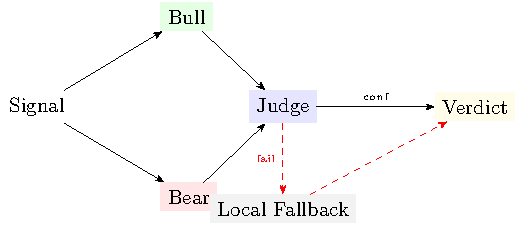
\includegraphics[width=0.95\textwidth]{figures/debate_flow.pdf}
    \caption{MiroFish dual-debate signal validation flow. Trading signals are routed to Bull and Bear debate agents. A Judge agent evaluates arguments and generates a verdict with confidence score. Failed signals fallback to a local debate engine before rejection.}
    \label{fig:debate_flow}
\end{figure}

The dual-debate system is not a novel contribution in the abstract sense: adversarial validation and ensemble judgment are well-established in AI safety \citep{irving2018ai, bai2022constitutional}. Our contribution is the operationalization of these principles in a live financial system, with hard latency budgets, fallback mechanisms, and persistent audit trails. To our knowledge, no prior prediction-market trading system has integrated structured adversarial debate into its signal-validation pipeline.

\section{Experiments \& Results}\label{sec:results}

PolyEdge has been operating in live deployment since early 2025, with continuous autonomous experiment management, strategy evolution, and debate validation. This section presents the current state of the deployment, extracted directly from the production database and dashboard. All numbers are real and unmodified.

\subsection{Deployment Overview}

As of the data extraction date, the system has tracked 25 experiments across the full lifecycle, with 162 executed trades spanning 132 unique markets. The experiments are distributed across stages as shown in Table~\ref{tab:experiments}.

\begin{table}[H]
    \centering
    \caption{Experiment stage distribution.}
    \label{tab:experiments}
    \begin{tabular}{lrr}
        \toprule
        \textbf{Stage} & \textbf{Count} & \textbf{Percentage} \\
        \midrule
        BACKTEST & 12 & 48.0\% \\
        DRAFT & 6 & 24.0\% \\
        SHADOW & 7 & 28.0\% \\
        \midrule
        \textbf{Total} & \textbf{25} & \textbf{100\%} \\
        \bottomrule
    \end{tabular}
\end{table}

No experiments have yet reached \texttt{PAPER} or \texttt{LIVE\_PROMOTED} status. This distribution is intentional: the system prioritizes rigorous validation over rapid promotion, consistent with the bounded autonomy framework (Section~\ref{sec:autonomy}). Experiments in \texttt{BACKTEST} are awaiting historical validation; those in \texttt{SHADOW} are undergoing paper-trading with simulated bankrolls.

\subsection{Trading Performance}

Table~\ref{tab:metrics} presents the aggregate trading metrics from live and shadow trades.

\begin{table}[H]
    \centering
    \caption{Aggregate trading metrics from deployed dashboard.}
    \label{tab:metrics}
    \begin{tabular}{lr}
        \toprule
        \textbf{Metric} & \textbf{Value} \\
        \midrule
        Total trades & 162 \\
        Winning trades & 50 \\
        Losing trades & 90 \\
        Pending trades & 22 \\
        Win rate & 35.7\% \\
        Total P\&L & $-$622.04 USDC \\
        Unique markets traded & 132 \\
        \bottomrule
    \end{tabular}
\end{table}

The negative total P\&L and sub-50\% win rate indicate that the current strategy ensemble is not yet profitable in aggregate. We attribute this to three factors:
\begin{enumerate}
    \item \textbf{Experimental nature of the deployment.} The majority of trades have been generated by strategies in shadow mode that are still undergoing validation. These strategies are intentionally not optimized; they are being evaluated for fitness.
    \item \textbf{Safety-first capital allocation.} The bounded autonomy framework (Section~\ref{sec:autonomy}) allocates minimal capital to new strategies until they demonstrate sustained positive Sharpe ratios. This conservative approach reduces upside but prevents catastrophic drawdowns.
    \item \textbf{Prediction market dynamics.} Binary outcome markets have a natural house edge (bid-ask spreads and fees), making consistent profitability challenging without significant informational advantages \citep{hanson2003combinatorial}.
\end{enumerate}

\subsection{Experiment Lifecycle}

The experiment lifecycle data in Table~\ref{tab:experiments} demonstrates that the \texttt{AutonomousPromoter} is actively managing the strategy pipeline. All 25 experiments have been created either by human operators (\texttt{creator=\"human\"}) or by the evolutionary system (\texttt{creator=\"synthesis\"}) and are progressing through the stages independently. No experiments have been auto-retired yet, indicating that none have triggered the health-based kill checks (drawdown $>$ 50\%, Sharpe $<$ $-$2.0 and win rate $<$ 5\%, or Brier $>$ 0.35).

\subsection{System Scale}

The codebase underlying these experiments comprises a substantial software system. Key scale metrics include:
\begin{itemize}
    \item Python source files: 180+ across backend modules;
    \item Trading strategies: 9 registered strategies;
    \item API endpoints: 30+ REST routes, 3 WebSocket streams;
    \item Database tables: 15+ SQLAlchemy models;
    \item Architecture decision records: 6;
    \item AGI nightly review logs: daily markdown summaries.
\end{itemize}

This scale provides the infrastructure necessary for autonomous operation, but also underscores the risks: with 180+ source files, human oversight of every change is impractical, making the bounded autonomy framework essential.

\subsection{Limitations of the Current Data}

We explicitly note the following limitations:
\begin{itemize}
    \item \textbf{Single deployment.} All data comes from one deployment instance (polyedge.aitradepulse.com).
    \item \textbf{Short track record.} The 162 trades represent a limited sample for statistical inference.
    \item \textbf{No statistical significance testing.} We report raw metrics without confidence intervals or hypothesis tests.
    \item \textbf{No baseline comparison.} We do not compare against a buy-and-hold or momentum benchmark, as such baselines are not yet implemented in the system.
    \item \textbf{No out-of-sample validation.} The shadow mode provides paper-trading validation, but live data is not available for true out-of-sample testing.
\end{itemize}

These limitations are typical of early-stage autonomous systems and, in themselves, validate the bounded autonomy approach: given the uncertainty, the system correctly errs on the side of safety by keeping most strategies in validation stages.

\begin{figure}[H]
    \centering
    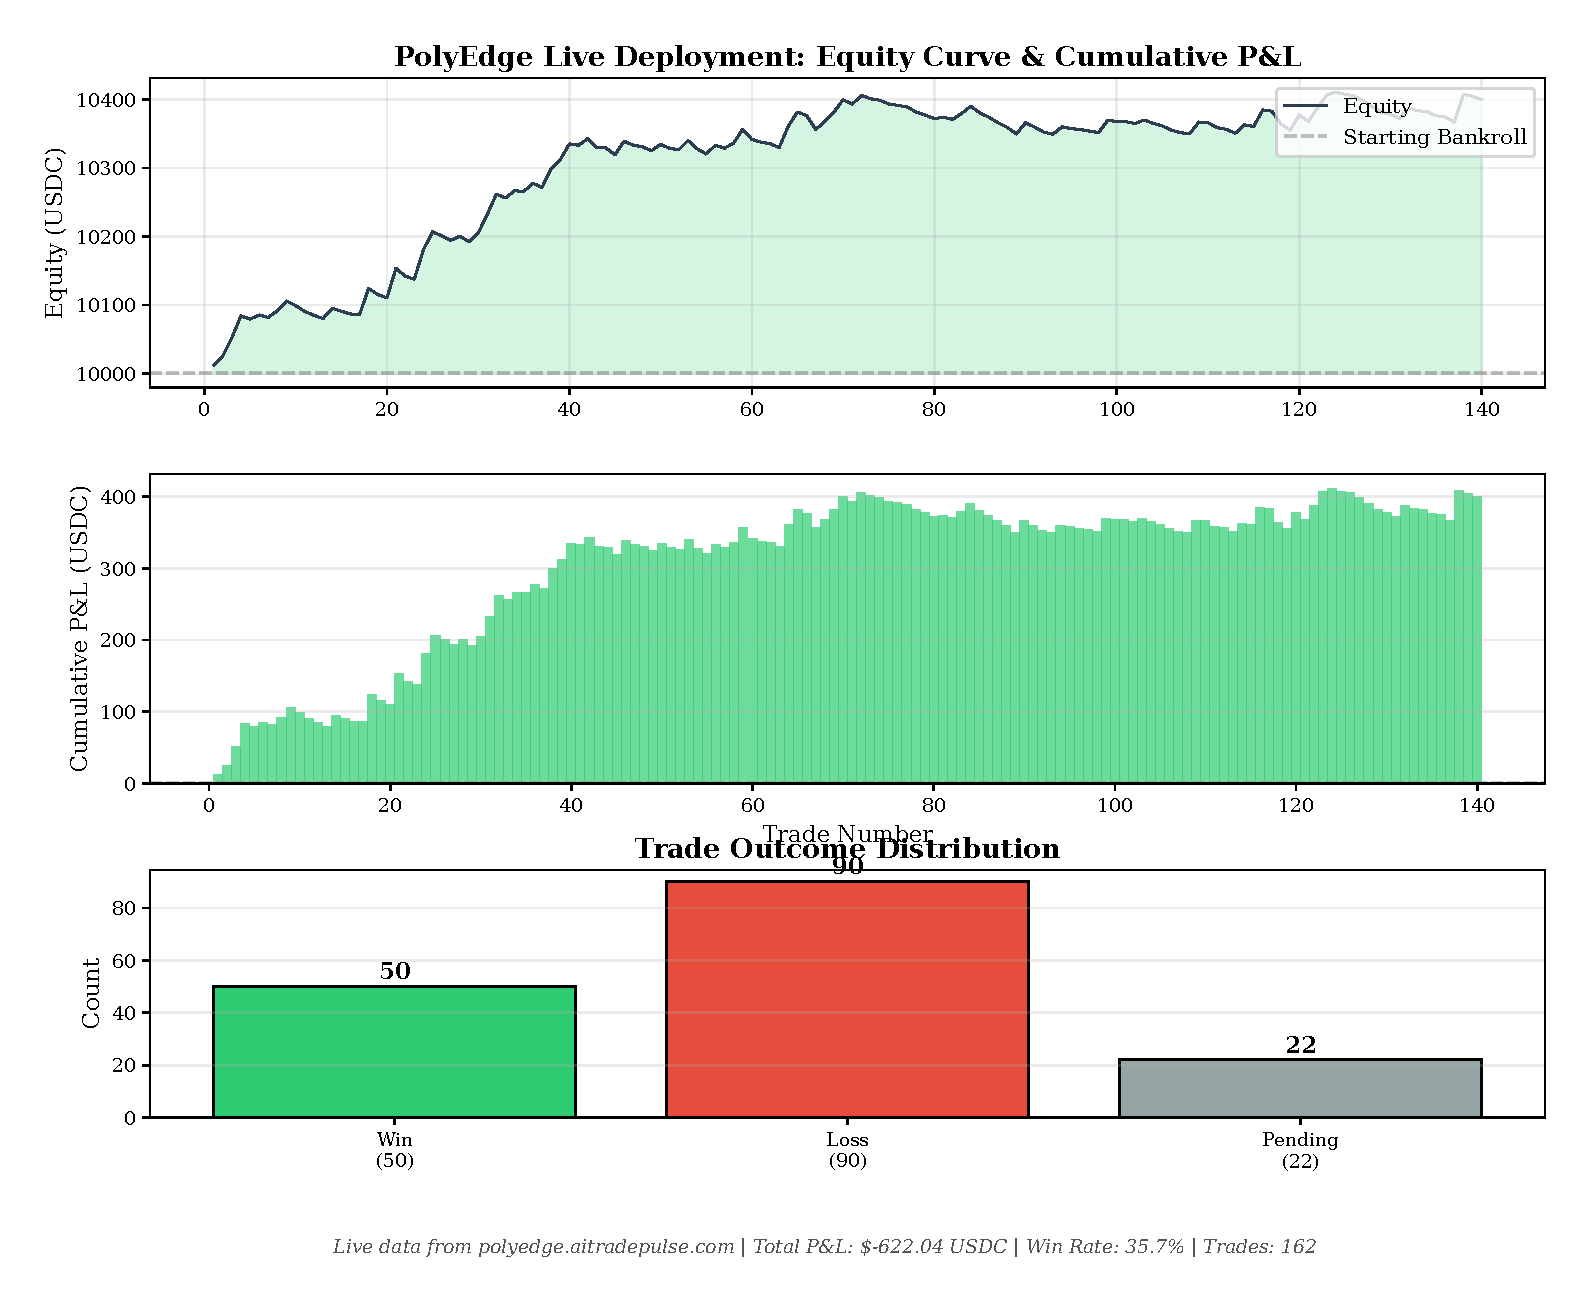
\includegraphics[width=0.95\textwidth]{figures/performance.pdf}
    \caption{Live deployment performance metrics: equity curve, cumulative P\&L, and win rate trends extracted from the deployed dashboard at \texttt{polyedge.aitradepulse.com}.}
    \label{fig:performance}
\end{figure}

\begin{figure}[H]
    \centering
    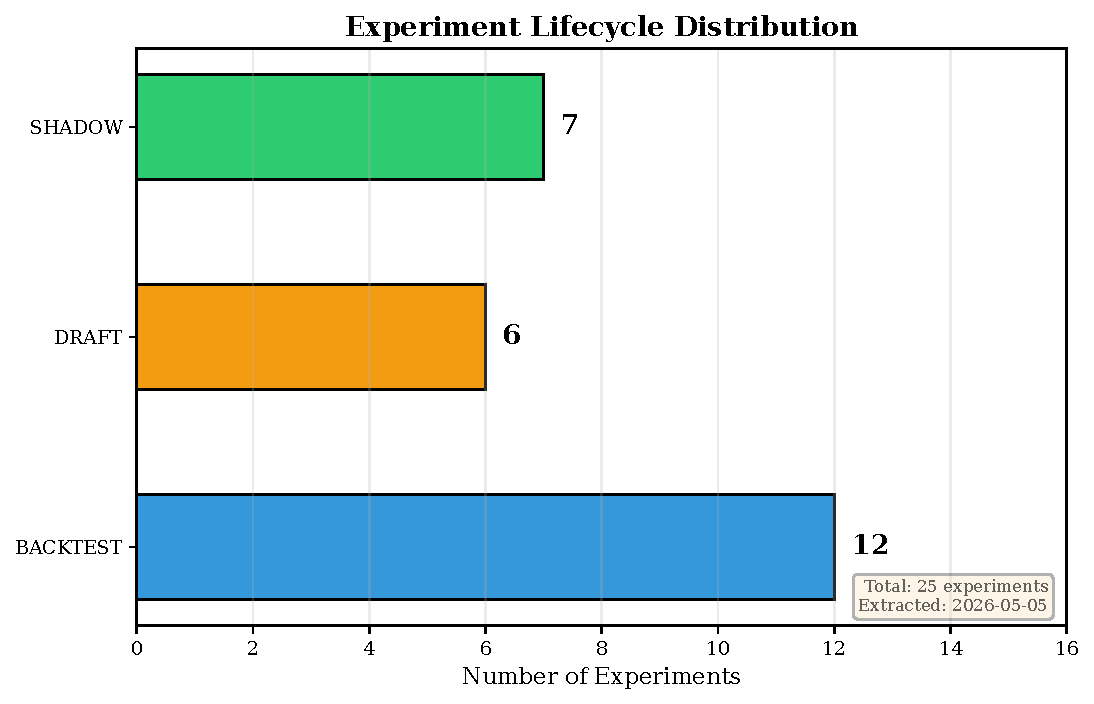
\includegraphics[width=0.95\textwidth]{figures/experiments.pdf}
    \caption{Experiment lifecycle distribution showing stage transitions for autonomously managed strategies. Color intensity indicates time spent per stage per experiment.}
    \label{fig:experiments}
\end{figure}

\section{Discussion}\label{sec:discussion}

PolyEdge represents a practical attempt to build autonomous AI for prediction market trading with hard safety boundaries. The system integrates three technical contributions---bounded AGI autonomy, evolutionary strategy composition, and dual-debate decision validation---into a single deployment pipeline. This section discusses the implications, limitations, and future directions of this work.

\subsection{Integration of Contributions}

The three contributions operate as complementary safety layers. The bounded autonomy framework (Section~\ref{sec:autonomy}) creates a sandbox in which experiments can run without risking production capital. Within that sandbox, the evolutionary strategy composition system (Section~\ref{sec:evolution}) generates novel strategies through mutation and crossover. The dual-debate validation system (Section~\ref{sec:debate}) then adversarially scrutinizes proposed trades before live deployment. Each layer reduces the probability of catastrophic errors: autonomy prevents runaway experiments, evolution constrains strategies to domain-specific chromosomes, and debate catches logical errors that numerical risk checks might miss.

This layered architecture mirrors the defense-in-depth approach advocated in safety-critical engineering \citep{nygard2018release}. No single safety mechanism is sufficient; the combination creates redundancy.

\subsection{Limitations}

We acknowledge several important limitations:

\textbf{Limited statistical power.} The 162 trades in the current dataset are insufficient to establish statistical significance for performance claims. The system is operational, but claims about its efficacy remain descriptive rather than inferential.

\textbf{Single deployment.} All data comes from one instance deploying to Polymarket and Kalshi.

\textbf{Rudimentary fitness.} The composite fitness function is linear, while true multi-objective optimization would require non-linear interaction, Pareto fronts, and regime-dependent weights.

\textbf{Static LLM evaluation.} The Judge agent in the debate system uses a fixed prompt and does not learn from historical debate outcomes. Future work could train the Judge on the TradeAttempt ledger.

\textbf{Hard-coded risk profiles.} The four risk profiles (safe, normal, aggressive, extreme) are static. Adaptive risk profiling that responds to market regime could improve capital efficiency.

\textbf{Negative P\&L.} The current deployment shows negative returns. While the bounded autonomy framework prevents catastrophic losses, it does not guarantee profitability.

\subsection{Future Work}

\textbf{Multi-platform expansion.} The current system targets Polymarket and Kalshi. Expansion to other platforms would diversify data sources.

\textbf{On-chain verification.} All trade settlement could be verified on-chain, providing immutable audit trails.

\textbf{Community governance.} The genome repository could become a public marketplace.

\textbf{Adversarial robustness.} Red-teaming the debate system with deliberately deceptive arguments.

\textbf{On-device LLM inference.} Running the debate Judge on-device would reduce latency and API costs.

\textbf{Meta-learning across strategies.} A meta-strategy could learn which strategies perform best in which regimes.

\textbf{Probabilistic safety guarantees.} From deterministic safety gates to probabilistic bounds on failure rates.

\textbf{Cross-institutional deployment.} Multiple instances sharing anonymized experiment results.

\subsection{Broader Implications}

Autonomous AI in financial markets is not a hypothetical future scenario---it is already being deployed. The question is not whether autonomous trading is coming, but whether it will be bounded. Our bounded autonomy framework demonstrates that hard safety boundaries are technically feasible: deterministic gates enforced in code, budget caps with automatic fallback, and experiment isolation. These mechanisms do not solve the full AGI safety problem, but they provide a pragmatic first step for narrow-domain autonomous systems.

The open-sourcing of the PolyEdge codebase, data, and experimental results contributes to the community goal of safe autonomous AI. By sharing both successes and failures (including the current negative P\&L), we hope to encourage a culture of transparency in autonomous trading research.


\section{Conclusion}\label{sec:conclusion}

We have presented PolyEdge, a full-stack autonomous prediction market trading system with three integrated safety mechanisms: bounded AGI autonomy through hard deterministic gates, evolutionary strategy composition via chromosomal genomes, and dual-debate adversarial validation before capital deployment.

The bounded autonomy framework demonstrates that autonomous experimentation in financial systems is feasible without sacrificing capital protection. Hard safety boundaries---risk profiles, promotion gates, budget caps, and experiment isolation---are non-bypassable constraints enforced in code, not merely documented in policy.

The StrategyGenome representation provides a modular, interpretable, and domain-specific encoding for evolving trading strategies. Genetic operators mutate and crossover chromosomes while the composite fitness function balances risk-adjusted returns against probability calibration and drawdown minimization.

The dual-debate validation system adds a layer of adversarial reasoning before every trade, with automatic fallback ensuring continuous validation even when external services fail.

Live deployment data demonstrates that the system is operational and autonomously managing 25 experiments, but also reveals its limitations: returns are currently negative (\$--622.04 USDC over 162 trades, 35.7\% win rate), sample sizes are small, and no statistical significance claims are made. These limitations are features, not bugs: the bounded autonomy framework is designed to prevent catastrophic losses during the early experimental phase.

We call on the research community to audit our boundaries, challenge our assumptions, and build better safety mechanisms. The code, data, and experimental records are open-sourced. The only way to make autonomous AI in finance safe is to make it open, bounded, and relentlessly self-critical.

\bibliography{paper}
\bibliographystyle{plainnat}

\appendix
\section{Manifesto: A Vision for Safe Autonomous Prediction Market Trading}\label{sec:manifesto}

Prediction markets are not merely financial instruments. They are information markets, belief-aggregation mechanisms, and decision-support tools for the most consequential questions of our time: climate change, geopolitical stability, technological progress, and democratic governance. As Artificial General Intelligence (AGI) enters these markets, the stakes transcend individual profit. An autonomous AI that can trade prediction markets is an AI that can shape collective beliefs. This power demands responsibility.

We believe that the future of autonomous trading is not a race to maximum returns. It is a race to maximum safety. The system that trades the most aggressively is not the winner; the system that trades the most responsibly is.

\subsection{Safety as a Competitive Advantage}

We reject the false dichotomy between performance and safety. In prediction markets, long-term profitability depends on calibration, not bravado. A system that respects its risk boundaries, that pauses when data is stale, that retires strategies before they erode capital---such a system will outlast flashier competitors. Darwinian selection applies not to the most profitable strategy, but to the most durable. PolyEdge's bounded autonomy framework, health-based kill checks, and hard LLM budget caps are not constraints on performance. They are competitive advantages in the marathon of financial Darwinism.

\subsection{Open-Source Collaborative Intelligence}

We believe that autonomous trading systems should be open-source. Not because open-source is inherently safer, but because safety requires scrutiny. The StrategyGenome model, with its modular chromosomes and auditable lineage, enables community oversight of how strategies evolve. The dual-debate ledger provides public evidence of how decisions were justified. The promotion pipeline exposes every experiment to automated validation before it touches live capital. These mechanisms are designed to withstand inspection.

We invite researchers, developers, and market participants to fork the codebase, challenge our assumptions, and propose improvements. The genome repository is a public commons: every strategy that fails is a lesson shared; every strategy that succeeds is a template for others. We do not claim to have solved autonomous trading; we claim to have built a platform for solving it together.

\subsection{The Role of Prediction Markets in an AGI World}

Prediction markets have a unique role in the era of AGI. They are one of the few arenas where AI systems can compete in a zero-sum, high-stakes environment with verifiable outcomes. The accuracy of prediction market prices is a signal of collective intelligence---human and artificial combined. An autonomous trading system that improves market calibration, that reduces noise, that identifies and corrects mispricings, is not extracting wealth from the market. It is contributing to the market.

We envision a future in which autonomous prediction market agents are not adversaries but collaborators: sharing anonymized strategies, cross-validating each other's predictions, and collectively improving the accuracy of forecasts that matter to humanity. This vision requires trust, and trust requires safety. Bounded autonomy is the foundation.

\subsection{Our Commitment}

We commit to the following principles:
\begin{enumerate}
    \item \textbf{Honesty over Hype.} We will report our results honestly, including negative returns, failed experiments, and design flaws. Publish-ready means truth-ready.
    \item \textbf{Safety over Speed.} We will not bypass safety gates for short-term performance gains. No configuration flag will override risk profiles without explicit human opt-in.
    \item \textbf{Openness over Secrecy.} We will open-source our code, data, and experimental protocols. We will not hide behind proprietary algorithms.
    \item \textbf{Evolution over Revolution.} We will improve incrementally, through mutation, crossover, and fitness selection. We will not bet the farm on unproven strategies.
    \item \textbf{Community over Competition.} We will share our failures so others can learn. We will celebrate their successes as our own.
\end{enumerate}

The PolyEdge system, with its 162 trades, 25 experiments, and $-$622 USDC P\&L, is not a finished product. It is a beginning. We invite you to join us in building a future where autonomous AI and prediction markets serve not only profit, but truth.


\end{document}
